\documentclass{article}
\usepackage{graphicx}
\usepackage{float}
\usepackage{caption}
\usepackage{subcaption}
\usepackage{setspace}
\usepackage{geometry}

\begin{document}

\title{Past Presidential Elections Results}

\maketitle

\begin{figure}[H]
    \centering
    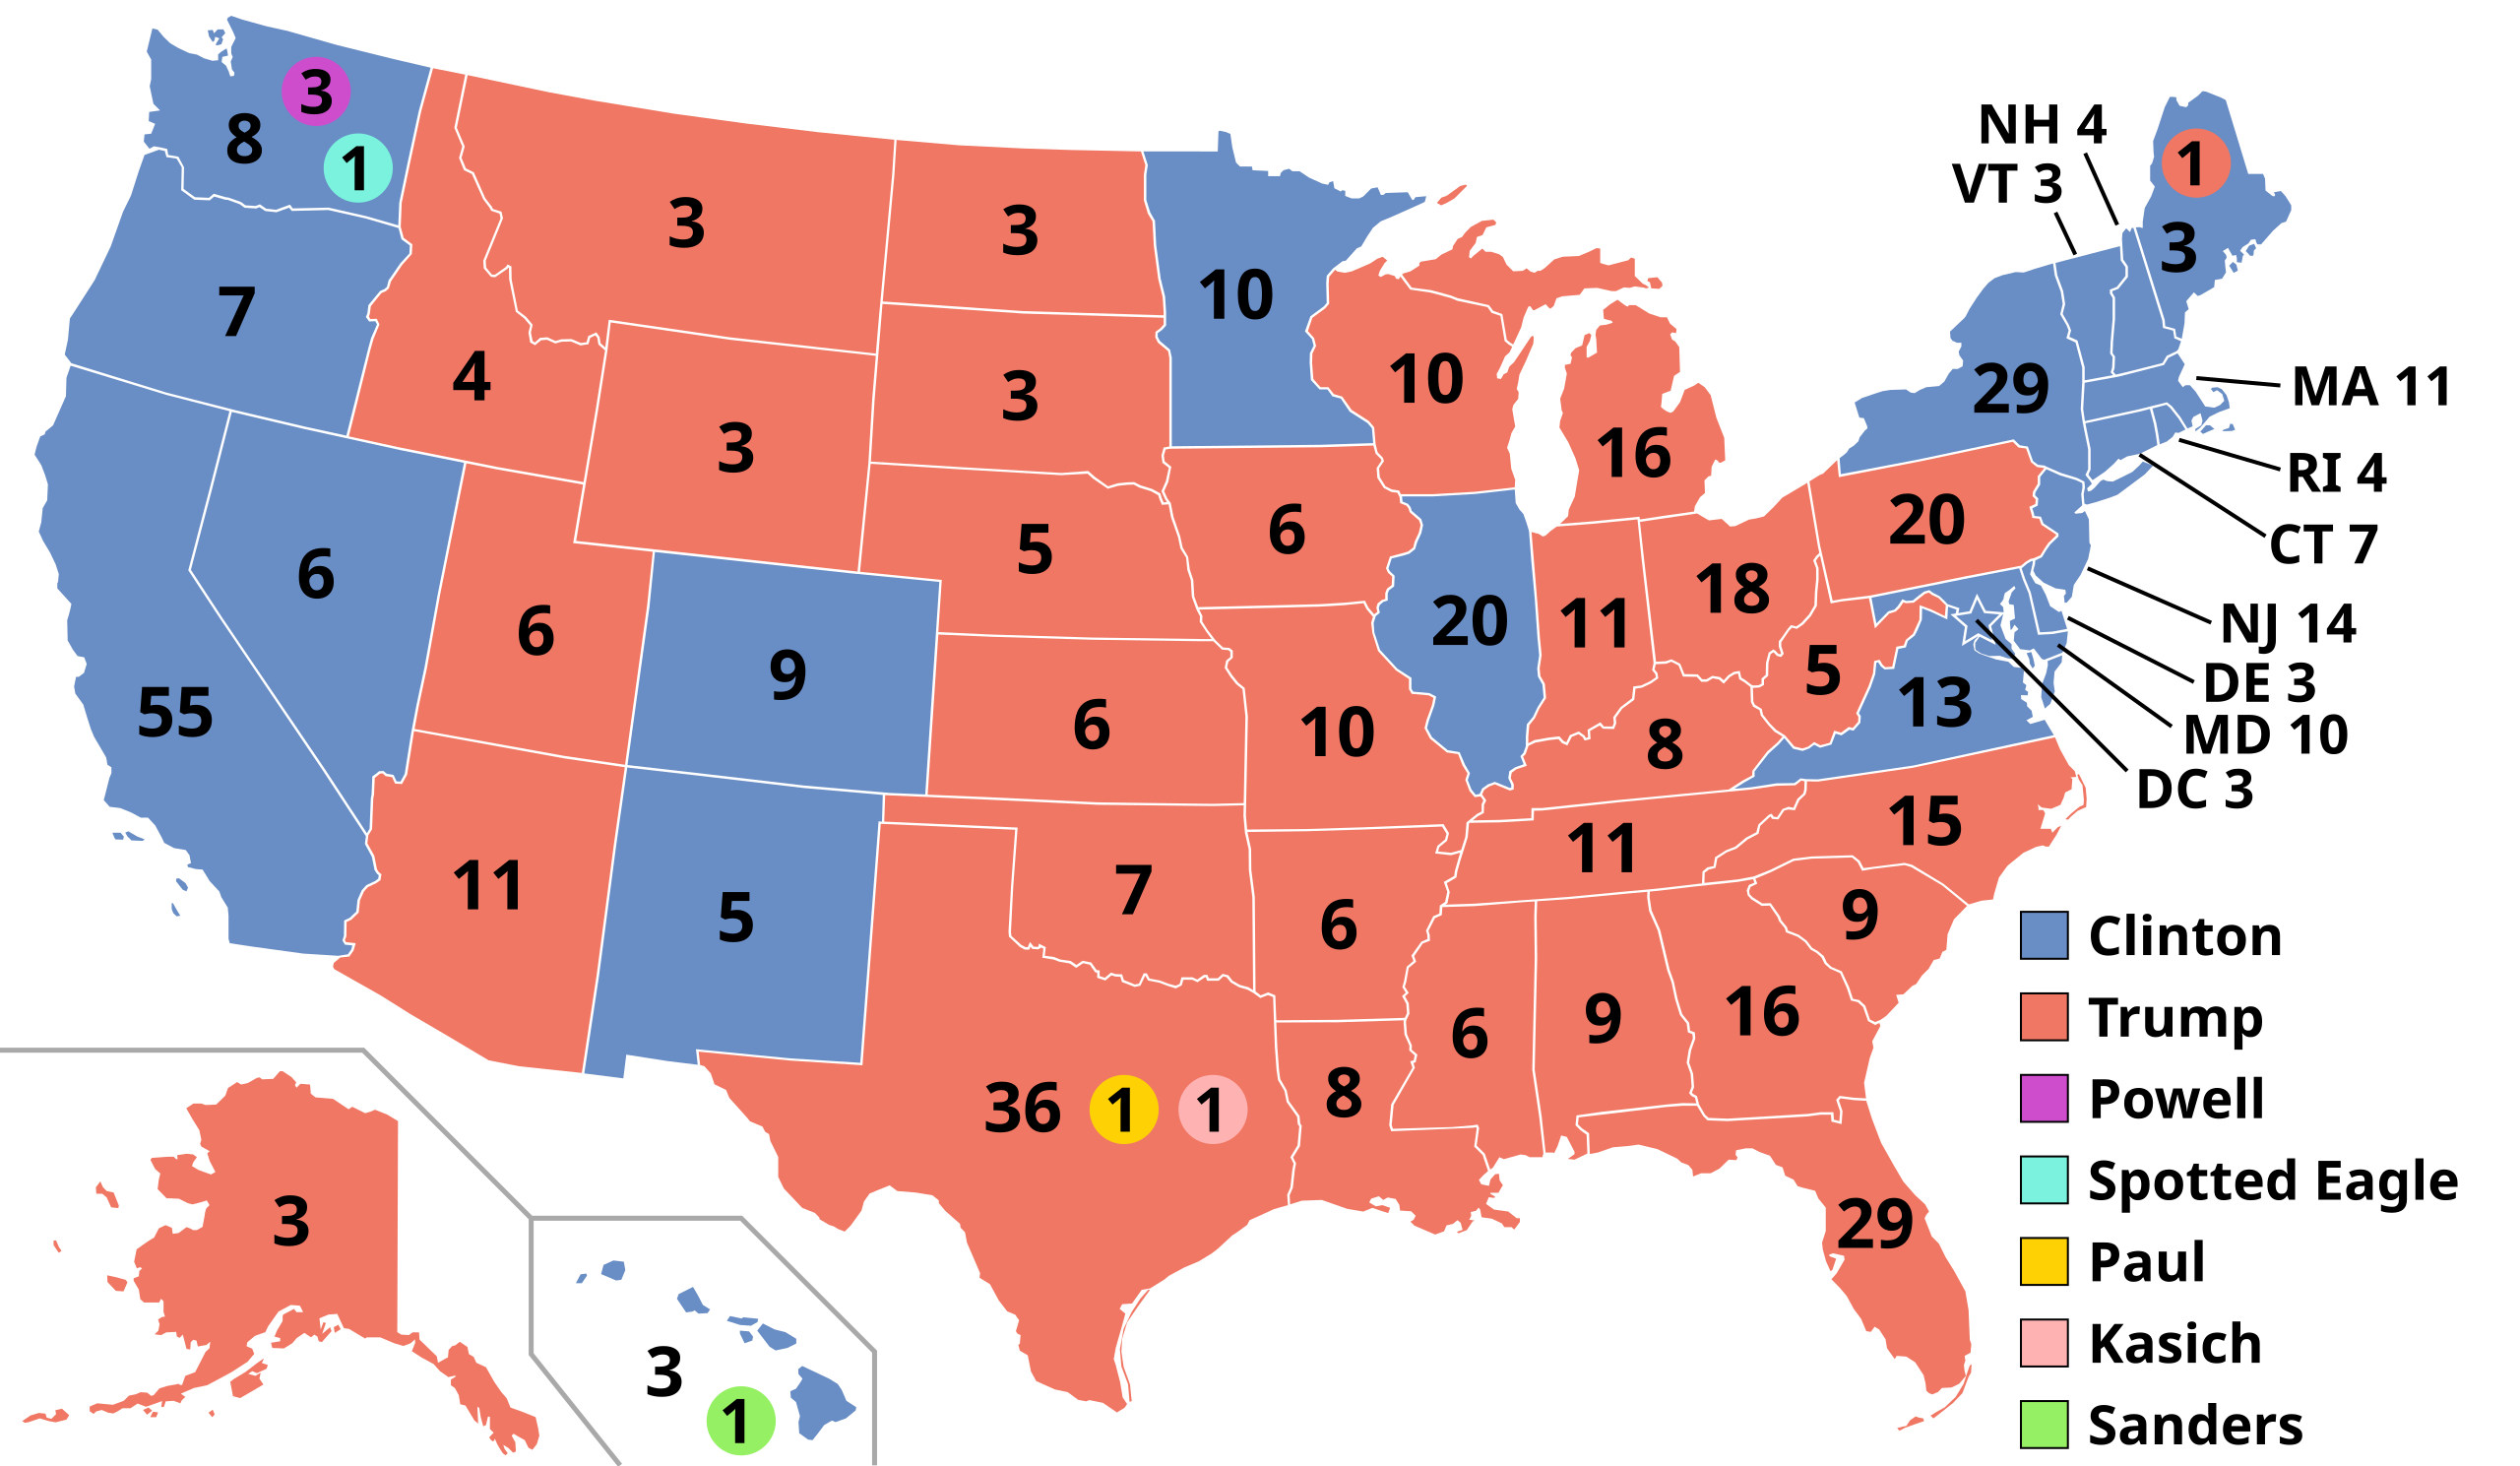
\includegraphics[width=0.6\textwidth]{ElectoralCollege2016.svg.png}
    \caption{Past presidential elections results in 2016}
    \label{fig:past_elections_2016}
\end{figure}

\begin{figure}[H]
    \centering
    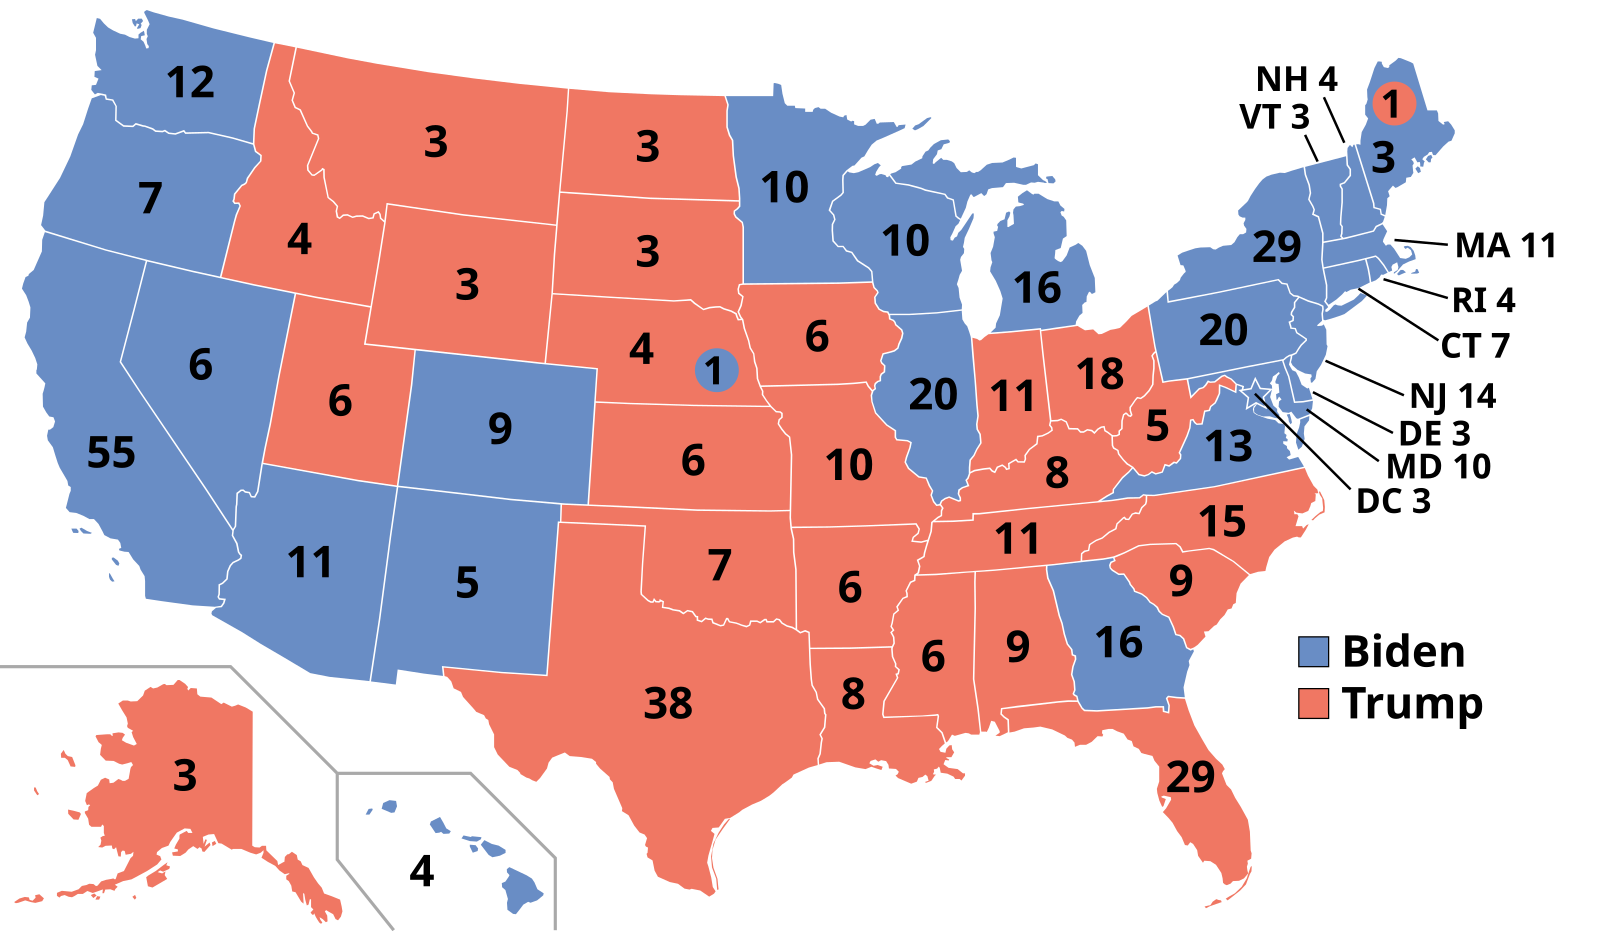
\includegraphics[width=0.6\textwidth]{ElectoralCollege2020.svg.png}
    \caption{Past presidential elections results in 2020}
    \label{fig:past_elections_2020}
\end{figure}

Presidential election results maps for the 2016 (figure \ref{fig:past_elections_2016}) and 2020 (figure \ref{fig:past_elections_2020}) elections. 
Red denotes states won by Trump and blue denotes those won by Clinton (2016) or Biden (2020). 
Numbers indicate electoral votes cast by each state and the District of Columbia. 

\end{document}

